\documentclass{article}

\usepackage[utf8]{inputenc}
\usepackage[T1]{fontenc}
\usepackage[greek,english]{babel}
\usepackage{alphabeta}
\usepackage{amsmath}
\usepackage{amssymb}
\usepackage{graphicx}
\usepackage{subcaption}
\usepackage{epstopdf}
\usepackage[margin=1in, paperwidth=7.5in,paperheight=10.5in]{geometry}


\newcommand\course{ΤΗΛ513}
\newcommand\courseName{Δορυφορικές Ζεύξεις}
\newcommand\semester{Εαρινό 2020}
\newcommand\assignmentNumber{Lab 3 Δορυφορικών Επικοινωνιών}
\newcommand\studentName{Μαυρογιώργης Δημήτρης}                           
\newcommand\studentNumber{2016030016}

\title{\underline{\textbf{\assignmentNumber}}} 
\author{\textsc{\textbf{Όνομα:}}  \studentName\\
		\textsc{\textbf{ΑΜ:}}  \studentNumber\\
		\course \ - \courseName\\ 
		\textsc{Πολυτεχνείο Κρήτης}
}
\date{\today}
\begin{document}
	\maketitle
\section{Εισαγωγή}
Σκοπός της άσκησης είναι η γνωριμία με τον αλγόριθμο Viterbi και η εφαρμογή του για το detection μιας ακολουθίας Ν συμβόλων MSK στο δέκτη.\\
Πιο συγκριμένα, ο αλγόριθμος Viterbi βρίσκει ένα μονοπάτι από την αρχή του trellis ως το τέλος του, το οποίο μεγιστοποιεί το αθροιστικό κόστος. Η βασική  ιδέα του αλγορίθμου είναι ότι ξεκινότανς από αριστερά προς τα δεξιά του trellis, οι μεταβάσεις προς μια κοινή κατάσταση σε οποιοδήποτε ενδιάμεσο βήμα, θα πρέπει να μεγιστοποιούν το συνολικό βάρος του μονοπατιού μέχρι την καάσταση αυτή.
Για παράδειγμα, αν υπάρχουν δύο καταστάσεις $x_{k-1}^{(1)}$ και $x_{k-1}^{(2)}$ με συνολικό βάρος μονοπατιού ως τις καταστάσεις αυτές $Γ(x_{k-1}^{(1)})$ και $Γ(x_{k-1}^{(2)})$ αντίστοιχα, τότε η μετάβαση $(x_{k-1}^{(1)},x_{k})$ είναι προτιμητέα της $(x_{k-1}^{(2)},x_{k})$ αν ισχύει το εξής:
$$Γ(x_{k-1}^{(1)}) + w(x_{k-1}^{(1)},x_{k}) > Γ(x_{k-1}^{(2)}) + w(x_{k-1}^{(2)},x_{k})$$

\section{Eρώτημα 1}
Το διακριτό σήμα βασικής ζώνης της MSK μπορεί να εκφραστεί ως εξής:
$$ r_{n} = 
\begin{bmatrix}
r_{1} \\
r_{2}
\end{bmatrix} = 
s_{n} + \begin{bmatrix}
			n_{1,n} \\
			n_{2,n}
		\end{bmatrix} (1), \  \  
s_{n} = s^{x_{n}}e^{jφ[n]}, $$
$$ 
φ[n+1] = φ[n] + x_{n}\frac{π}{2}, n = 1, 2, \dots N, \ \  φ[1] = 0
$$
με $n_{1,n} \texttt{\char`\~} CN(0,2β)$, $n_{2,n} \texttt{\char`\~} CN(0,2β)$, $n_{1,n}$ ανεξάρτητο του $n_{2,n}$ και ανεξαρτησία μεταξύ $n_{1,n}$, $n_{2,n}$ και $n_{1,m}$, $n_{2,m}$ για $n \ne m$. Τα σταθερά διανύσματα ${s_{n}}$ για $x_{n} \in { \pm 1}$ είναι τα εξής:
$$s^{-1} = 
\begin{bmatrix}
-\frac{2A\sqrt{T}j}{π} \\ 
\frac{A\sqrt{T}\sqrt{π^{2}-4}}{π}
\end{bmatrix}, \  \  \  
s^{1} = 
\begin{bmatrix}
	A\sqrt{T} \\ 
	0
\end{bmatrix}
$$
Επίσης, ορίζουμε το SNR ως εξής:
$$SNR = \frac{A^2T}{β}$$
Για SNR=5 dB, προσομοιώνουμε την εξίσωση (1), εφορμόζοντας τον αργόριθμο Viterbi και προέκυψε ότι το BER με τη χρήση Viterbi είναι περίπου 0.0727, ενώ με τη μέθοδο που υλοποιήθηκε στο LAB1 είναι περίπου 0.0729. \\
Συνεπώς, ο αλγόριθμος Viterbi μας έδωσε σχεδό το ίδιο BER με αυτό της υλοποίησης του 1ου εργαστηρίου.
\section{Eρώτημα 2}
Για τιμές SNR=6 εως 12 dB προκύπει το παρακάτω αποτέλεσμα προσομοίωσης για τον αλγόριθμο Viterbi:\\
\begin{figure}[h]
	\centering
	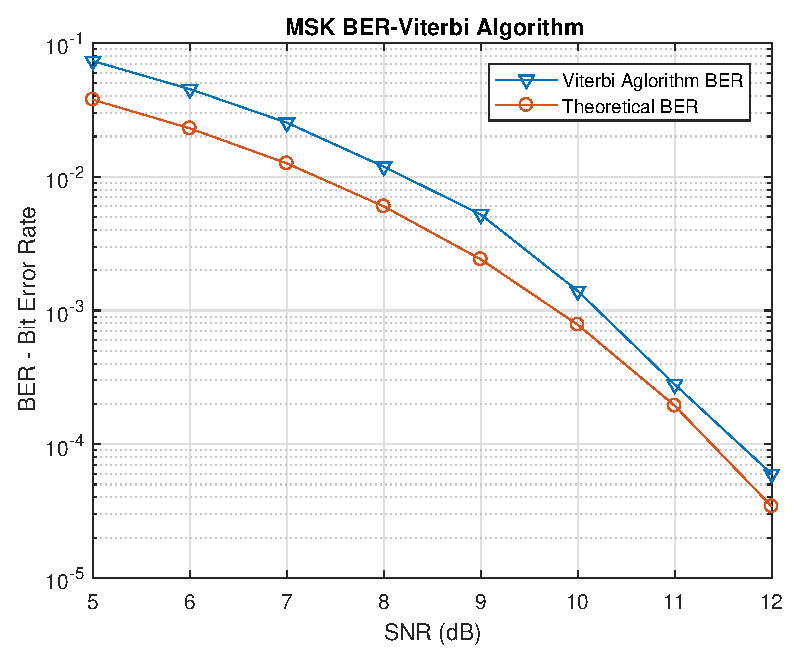
\includegraphics[width=0.5\linewidth]{./results/epsFig2}
	\caption{SNR(dB)-BER with Viterbi Algorithm}
\end{figure}
\section{Eρώτημα 3}

\begin{figure}[h!]
	\centering
	\begin{subfigure}[t]{0.5\textwidth}
		\centering
		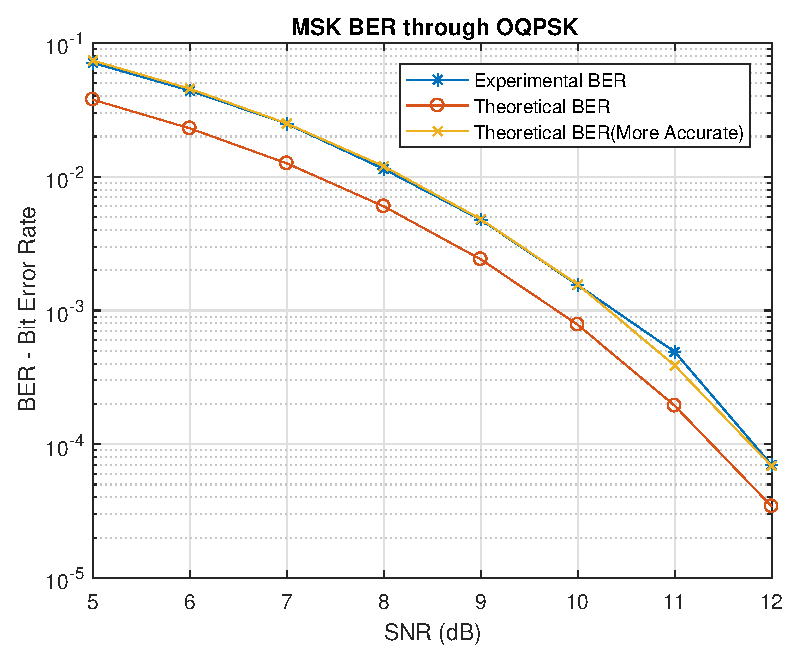
\includegraphics[width=\linewidth]{./results/epsFig1}
		\caption{Theoritical-LAB1-Viterbi BER}
	\end{subfigure}%
	~
	\begin{subfigure}[t]{0.5\textwidth}
		\centering
		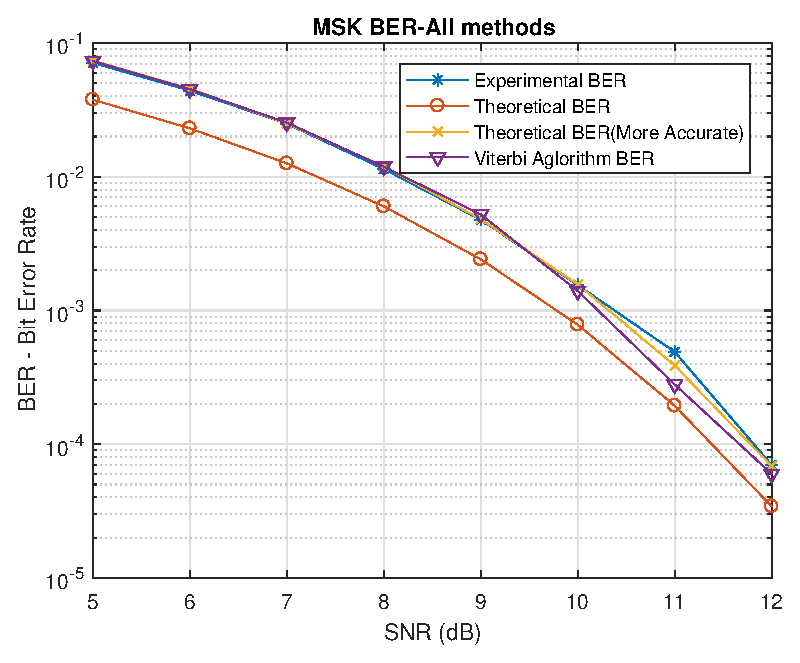
\includegraphics[width=\linewidth]{./results/epsFig3}
		\caption{Theoritical-Lab1-Viterbi- Theritical(More Accurate) BER}
	\end{subfigure}
\end{figure}
\noindent
Από τα διαγράμματα που παρουσιάστηκαν παραπάνω συμπαραίνουμε ότι o αλγόριθμος Viterbi και η μέθοδος του Lab1 για detection στο δέκτη δίνουν σχεδόν το ίδιο BER, καθώς οι πειραματικές τους κυματομορφές σχεδόν ταυτίζονται. \\
Eπίσης, οι δύο αυτές μέθοδοι δίνουν ένα BER το οποίο είναι λίγο χειρότερο από $Q(\sqrt{SNR})$. \\
Tέλος, αξίζει να σημειωθεί ότι τόσο ο αλγόριθμος Viterbi, όσο και η μέθοδος του Lab1 έχουν ακριβές ΒER, το οποίο ισούται με $2 \cdot  Q(\sqrt{SNR}) - [Q(\sqrt{SNR})]^2$, όπως είχε αποδειχτεί στο Lab1

\end{document}
